% !TEX root = ../main.tex

\chapter{Malware Analysis}
\label{chap:1}

\daniele{Add introductory text on the importance of having efficient and semantically rich techniques for analyzing malware, the different trade-offs for different levels of inspection, and the heterogeneous alternatives available}

The goal of malware analysis is to analyze a suspicious binary to determine its functionalities and extract very specific behaviour patterns that can help identify the presence of such binary in the network. This collection of interactions between the sample and the environment is called Indicator of Compromise (IoC).

There are many different methods that can be used for malware analysis however they fall into two main categories: Static and Dynamic analysis. 

\noindent
\begin{figure}[htp]
\centering
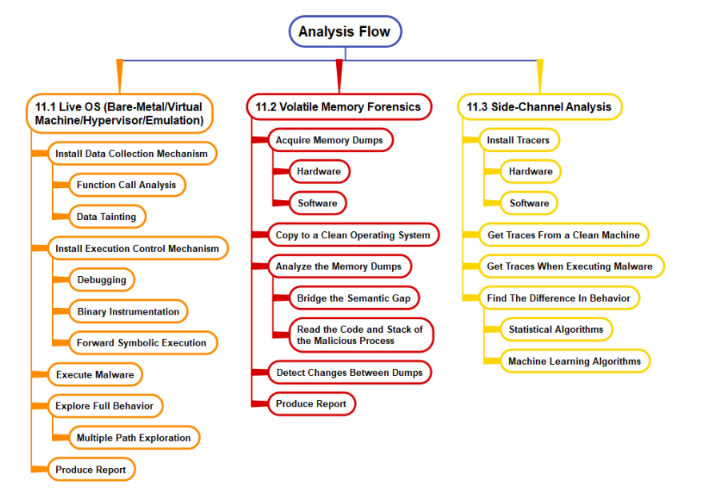
\includegraphics[width=\linewidth]{images/dynanalysis.png}
\caption{Malware analysis techniques}
\label{fig:mat}
\end{figure}

\section{Static and Dynamic Approaches}
There are two types of analysis techniques that can be used to fully understand and dissect a malicious piece of code.

\subsection*{Static Analysis (and Its Challenges)}

\textit{Static analysis} is the process of analyzing a, possibly, malicious piece of software without running it on the machine. This is usually done with the aid of different tools to parse the header of the executable and to extract as many information as possible. Subsequently the malware can be analyzed using a disassembler which is a program that allows the user to take the machine code and "reassemble" it to a higher level, human readable, code. Such process can be taken even further with the use of a decompiler, this software tries to bring a higher level of abstraction into the reversing process by decompiling machine code into a pseudo-language often similar to C reducing the effort required by the analyst to interpret machine code.

This kind of analysis is usually very time consuming and requires deep understanding of the underlying architecture of the processor. Moreover the malware author can use different techniques to modify the compiled code making it harder to reverse engineer or even to trick the analyst into believing that the code has different capabilities than the real ones. These techniques are commonly referred as \textbf{Obfuscation} however there are many different techniques that are used to hide malware capabilities: \textit{Encryption, Packing, Obfuscation, Polymorphism, Metamorphism}.\cite{Ye2017ASO}

\textit{Encryption} and \textit{Obfuscation} are similar techniques used to hide pieces of the malicious code not only from the analyst but also from antivirus software. At low level often \textit{Encryption} consists of performing a \textit{XOR} operation on a defined portion of memory while \textit{Obfuscation} involves masquerading API calls and split strings in the code in order to make it harder to understand the real behaviour of the malware.

On the other hand \textit{Packing} consists in encrypting and compressing the real code of the malware and, instead of shipping the "real" malicious code, the packed version will feature an unpacking stub which will take care of extracting and then running the malware directly into the memory making it harder to detect and reverse engineer.

Finally \textit{Polymorphism} and \textit{Metamorphism} are conceptually similar, the first one involves a polymorpic engine which allows to compile the code in a non deterministic way meaning that it will be different at each compilation but it will however still retain all the initial functionalities, this is usually achieved also with the use of encryption. \textit{Metamorphism} on the other hand is a really interesting technique through which the code of a program can be modified at run time adding a great layer of complexity and opening the door to a dedicated category of malware.

The Static Analysis is a powerful technique however for some more advanced pieces of malware it is not enough and instead it is required to run the malicious code in order to fully understand the capabilities and interactions with the machine.

\subsection*{Dynamic Analysis}

%\daniele{Too dry: your thesis is around dynamic analysis! Detail the different execution technologies available to date, and emphasize why whole-system emulation is important for fine-grained analysis of malware and in general for software security topics (e.g. for whole-system information flow tracking, you can cite the DECAF papers}

\textit{Dynamic analysis} is the process of running the malicious program in a controlled environment in order to collect as many information as possible about the behaviour of a specific program. There are different approaches that can be taken in order to perform an effective Dynamic analysis: diffing, monitoring, tracing and debugging. The more a method is comprehensive and powerful the less it is easy to use or to implement.

\begin{itemize}
    \item \textbf{Diffing} consists of comparing the difference between a clean system and one in which the malware has run. This is usually achieved on a virtual machine using snapshots. However this can be done also targeted on specific parts of the system such as the windows registry or important folders. In this way it is easy to find artifacts and manipulation left on the system by the malware such as persistence through the memory. On the other hand, however, this methods is not able to capture artifacts that are removed from the malware during execution.  
    
    \item \textbf{Monitoring} consists of carefully monitoring the system and capture every change on it or any network traffic that takes place after the malware is executed. In this way it is possible to have a complete overview of every action that the malware is performing on the machine. However, the data gathered in this way often have a great amount of noise and therefore needs to be filtered out and carefully examined to extract only relevant information.
    
    \item \textbf{Tracing} consists of hooking important API or System Calls in the system in order to capture important events. In this way however, it is possible to achieve a much deeper level of details compared to System Monitoring since it is possible to monitor each external function invoked on the system. Blending in Static and Dynamic analysis and providing useful information on the execution flow of the malware as well as on the low level interaction with the system. One of the disadvantages of this system is that it requires interpretation of the gathered information as well as to exclude data related to normal activity on the system.
    
    \item \textbf{Debugging} consists of attaching a specialized software to the malware and placing breakpoints in specific parts of the code in order to inspect the internal state of the program. This is particularly useful as it gives complete control over the execution of the malware therefore allowing to modify the internals of the machine such as processor registers, memory and so on. This approach however, requires to deeply understand the source code of the malware in order to identify the interesting execution branches and place breakpoints correctly. Malwares can easily check the presence of a debugger using a system call and can therefore change their behaviour accordingly, this poses further challenges to the analyst whom has to modify the environment to mask such artifact. 
    
\end{itemize}

It is of paramount importance in this phase that the machine on which the malware runs is isolated from the network. The ideal situation would be to have a real machine that can be used to run the malware and then re-imaged every time after the analysis is complete. This has obviously some huge pitfalls in terms of performance and efficiency therefore, the best way to perform Dynamic Analysis nowadays is using a virtual machine. Such virtual machines will need to be configured in order to have proper measures in place to avoid external communication and stop the malicious program from spreading to other machines in the network. 

Different level of analysis requires different amount of visibility and interaction with the environment. In particular, in order to extract as many information as possible from an analyzed system, it is necessary to have complete control of every single component. For this reason Virtual Machines created on a Full System Emulation environment are particularly suited for the job as they allow for fine grained control over the simulation. In such system it is possible to place custom pieces of code in very specific points of the simulated hardware. This practice, called instrumentation, allows the analyst to instrument not only the malware but also the environment itself, in this way the analysis can be performed at different levels making it more efficient, rich and also completely transparent for the malware.

For example Whole System Emulation allows the user to interact and control directly the emulated CPU making it easy to extract opcodes and make changes to a live program from outside the system. This is particularly important when analyzing malwares that attempt to detect and evade the analysis environment. 

Dynamic as well as Static Analysis must be carried out by a single person which must dedicated many hours into deeply understanding and dissecting the malicious code. Although this is highly reliable and produces a great amount of information it is not scalable or efficient. For this reason some ad-hoc solutions to carry out an initial triage have been developed. Such solutions are dedicated virtual machines, called sandbox, inside which it is possible to safely run the malware. The analysis framework will then take care of performing different types of analysis, from network traffic to registry interaction, in order to determine the nature of the executable. This is often referred as automatic malware analysis, some solutions will simply produce a report detailing all the actions performed on a system by a specific executable other will try to perform some further analysis on such data in order to understand if the binary is malicious or not. Nowadays the most common sandboxes are: cuckoo\footnote{\url{https://cuckoosandbox.org/}}, joe sandbox \footnote{\url{https://www.joesandbox.com/}}, any.run\footnote{\url{any.run}} and VMRay \footnote{\url{https://www.vmray.com/}}. Most of these solutions provides web based user interfaces through which it is possible to submit samples to the underlying system and retrieve results of the analysis. 

In most cases the best analysis technique is a combination of the Static and Dynamic ones. As a matter of fact debuggers are often used to unpack malware by setting breakpoints in the code and running it in a controlled environment until the real malware is extracted and loaded into memory, the resulting piece of code can then be dumped to disk and statically analyzed.

\subsection{Other possible approaches}

The two described method above requires that the analyst has acquired the executable of the malware and is able to dissect it on disk or run it in a safe environment. There are however some cases in which this is not possible, an example is file-less malware where the entire malicious code resides into memory and never touches the disk. In this case the analysis must be carried out on a snapshot of the system. 

There are two different approaches when creating a snapshot of the memory: one is dumping the entire content of the ram on disk and then carry out the analysis on it. This has many advantages as it will contain, most likely, all the information needed to carry out a complete analysis. Moreover, this will include also kernel structures that will be fundamental when trying to reconstruct the execution of the malware in memory. Moreover, from such memory dump, it is possible to select the memory region in which the malicious code resides and perform a Static analysis on it. The disadvantage of this technique is that the dump file will be of the same size of the ram and only a small portion of it will be really useful for the analysis making it harder to handle and slowing down some analysis tools. 

The volatility framework\footnote{https://github.com/volatilityfoundation/volatility} is the state of the art for this kind of analysis, it implements many different plugins that are capable of performing different types of analysis on a RAM dump file. 

The second approach consists of creating a Full Memory Dump of a single program. Such file, as opposed to the above mentioned one, will contain only the portion of memory reserved to the specified executable. In this way some information about the system, such as the kernel structures, are lost but the produced file will be much smaller. This portion of memory, most of the times, will contain enough information to carry out full malware analysis of the malicious code.   

\todo{has docker ever been used for malware analysis? \url{https://www.reddit.com/r/docker/comments/eakd50/help_can_i_safely_run_malware_inside_a_container/}
\url{https://ieeexplore.ieee.org/abstract/document/9042158}}

\daniele{On Linux they also use eBPF see for instance \url{https://github.com/aquasecurity/tracee}. There are approaches for bare-metal analysis, or with instrumentation done at firmware level (check the BluePill paper, there is a nice table and discussion of other methods)}

% take a look https://www.blackhat.com/docs/us-14/materials/us-14-Kruegel-Full-System-Emulation-Achieving-Successful-Automated-Dynamic-Analysis-Of-Evasive-Malware-WP.pdf
 
\section{Evasive Malware}
\label{sec:evmal}

As mentioned previously the Dynamic Analysis takes place inside a controlled environment. Having a real computer, isolated from the network and re-imaged every time that a sample is analyzed is the best scenario but also highly inefficient. There are different technologies, such as Virtual Machines, that are used nowadays to achieve the same results but with less effort, overhead and a great saving in terms of costs. 

From an attacker prospective detecting if the current machine is a physical one or a virtual one can really make the difference as the more it takes for an analyst to reverse a sample the more it can stay in the wild and perform malicious actions. In addition to this, testing for the presence of a debugger installed in the system or attached to the program is another form of protection that is used by the malware to avoid the analysis process.

\noindent
\begin{figure}[htp]
\centering
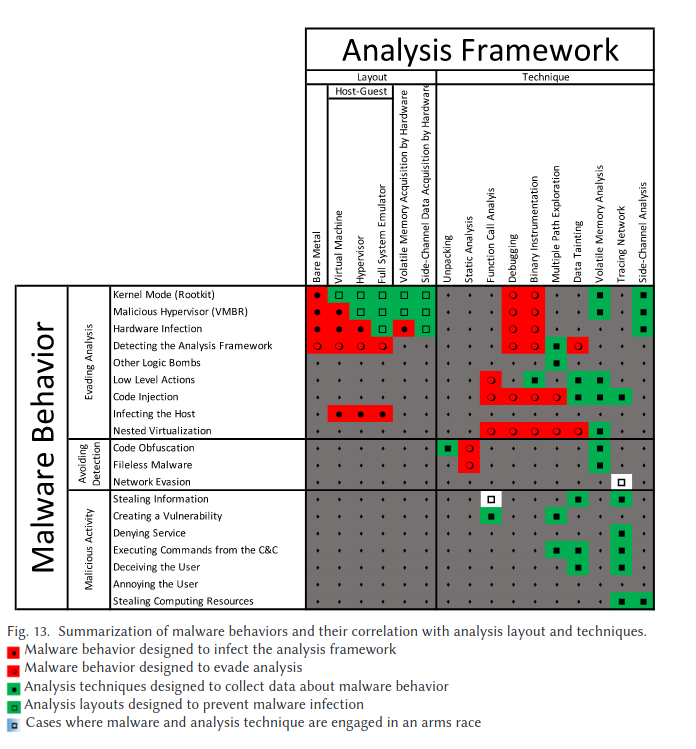
\includegraphics[width=\linewidth]{images/mal-fram.png}
\caption{Malware analysis techniques against various malware types}
\label{fig:mfrm}
\end{figure}

There are multiple techniques used to detect if a piece of code is running in an analysis environment. According to \cite{9018111} such techniques can be divided in two categories:
\daniele{Inaccurate: red pills originally detected emulators, but you should say that now you can use them to detect anomalies when executing instructions or looking up the position of specific structures in memory (see VMware artifacts) on a hypervisor or any other dynamic execution platform that is not a bare-metal machine}

\begin{enumerate}
    \item \textbf{Red Pills} used to detect if a CPU is emulated. As detailed in \cite{bruschi} these usually consists of different sets of opcodes that behaves differently depending if they are executed inside a physical or virtualized environment. However in addition to classical red pills emulators can also be detected by leveraging hypervisor calls such as CPUID and other particular instructions such as RDTSC.
    \item \textbf{Virtualization Artifacts} are peculiar characteristics of a machine that are introduced with virtualization. Most notably virtual machines, due to their nature, leave some distinctive fingerprints in the system.
\end{enumerate}

The CPUID instruction\footnote{\url{https://c9x.me/x86/html/file_module_x86_id_45.html}} (shorthand for CPU IDentification) is one of the most used and interesting \textbf{Red Pills} as it can produce a good amount of details about the processor and the environment in general.

CPUID reads the input parameter from the \textit{EAX} registry and places the outputs in the \textit{EAX, EBX, ECX, EDX} registries. The length of the result is variable and therefore different registers are used according to the initial \textit{EAX} value. From a virtualization detection prospective the most interesting results are obtained by calling this instruction with the \textbf{0x1}, \textbf{0x40000000} and \textbf{0x80000000}\cite{CPUID}. 

When calling \textit{CPUID} with 0x1 as parameter the CPU feature information are returned in \textit{ECX} and \textit{EDX}. The last 3 bits of the value in \textit{ECX} are reserved and the \nth{2} of those (i.e. the \nth{31}) bit is called Hypervisor bit, physical CPUs sets this bit to 0 while virtual ones set this bit to 1. This is a simple and fast way to detect if a program is running under a virtualized environment. 

In addition to this calling \textit{CPUID} with 0x40000000 as parameter will return the Hypervisor Brand information in \textit{EAX, ECX, EDX}. While calling \textit{CPUID 0x80000000} will return the CPU Brand information in the \textit{EAX, EBX, ECX, EDX} registries. Obviously both of the above information are set to specific values if the environment is virtualized. 

Another interesting instruction is \textit{RDTSC} \footnote{\url{https://c9x.me/x86/html/file_module_x86_id_278.html}} this is used to read the processor timestamp counter, which is a 64 bit values that stores the number of cpu cycles elapsed since the last reset. Lower bits are stored in the \textit{EDX} register while higher bits are stored in the \textit{EAX} register. The difference between two subsequent executions of this instruction on a physical CPU will be low while it will be a much higher number on virtual CPUs.

Both CPUID and RDTSC are privileged instructions, this means that they can only be executed in kernel mode, if they are executed in user mode the CPU will generate a trap. If such instructions are executed from inside a Virtual Machine a VM Exit event is generated and the control is given to the Hypervisor. Fingerprinting the time it takes to perform a VM Exit is another method used by evasive malware to detect the presence of a virtual machine. However it must be noted that RDTSC alone is not sufficient to reliably generate a VM Exit event, as a matter of fact this is a conditionally exiting instruction meaning that the event will be generated only under specific circumstances. On the other hand CPUID is an unconditionally exiting instruction and therefore a VM Exit will occur each time the instruction is executed. Therefore the mechanism used by malware to fingerprint the system consists in chaining a CPUID and RDTSC instruction and comparing it to a pure RDTSC run, if the difference is above a certain threshold then the presence of a virtual machine is detected.

On the other hand \textbf{Execution Artifacts} are very dependant on the virtualization system used and can be found in different places of the system. One of the most obvious artifact is the MAC Address of the network interfaces which, by default, is set to well known values by all the different Virtualization Software as in Figure \ref{fig:vms}.

\noindent
\begin{figure}[htp]
\centering
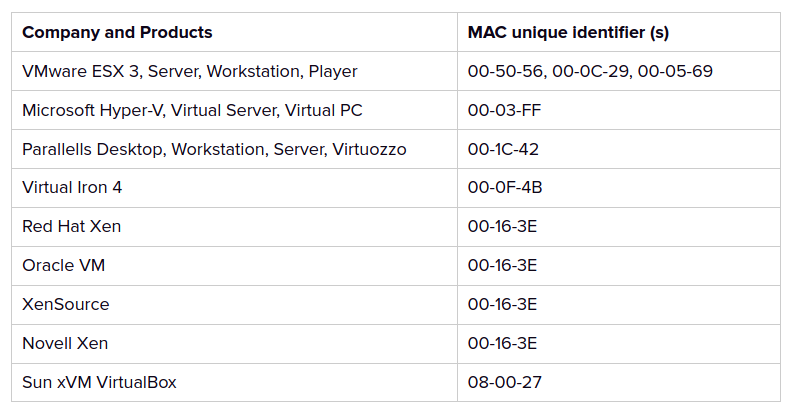
\includegraphics[width=\linewidth]{images/vms-mac-address.png}
\caption{Common VMs mac addresses \newline \url{https://www.techrepublic.com/blog/data-center/mac-address-scorecard-for-common-virtual-machine-platforms/}}
\label{fig:vms}
\end{figure}

Another common source of information for evasive malware is the windows registry, this is defined in the official documentation as a central hierarchical database used to store information that is necessary to configure the system for one or more users, applications, and hardware devices.

\textit{"The Registry contains information that Windows continually references during operation, such as profiles for each user, the applications installed on the computer and the types of documents that each can create, property sheet settings for folders and application icons, what hardware exists on the system, and the ports that are being used."}\cite{windocs}

The windows registry has a well defined structure, it is organized as a tree and each node in the tree is called a \textit{key}. Each \textit{key} in the registry can contain both \textit{sub-keys} and data entries called \textit{values}. Each \textit{key} has at least 1 value called \textit{Default}. The name of each \textit{key} consists of one or more characters and is case insensitive. Sometimes the presence of a \textit{key} it is sufficient for the application to store a certain setting, other times a \textit{key} will have different \textit{values} representing a piece of information. \textit{Values} can have many different types according to the information they are holding, the most common values are \lstinline{REG_BINARY, REG_DWORD} and \lstinline{REG_SZ}. 


An example of virtualization artifact related to the registry is the \textit{SystemBiosVersion} value which for VirtualBox and QEMU is as follows:
\begin{itemize}
    \item \lstinline{HARDWARE\Description\System (SystemBiosVersion) (VBOX)}
    \item \lstinline{HARDWARE\Description\System (SystemBiosVersion) (QEMU)} 
\end{itemize}

Other virtualization artifacts are system files and drivers such as, among the others:
\begin{itemize}
    \item \lstinline{system32\drivers\vmci.sys}
    \item \lstinline{system32\drivers\VBoxVideo.sys}
    \item \lstinline{system32\vboxtray.exe}
\end{itemize}

Moreover other structures like ACPI tables, SMBIOS strings as well as Disk Size and RAM Size can be used to fingerprint the system and reveal the presence of a virtual machine. 


\section{QEMU and Emulation Artifacts}
\daniele{give some context on QEMU, explain why relevant (you will say it in the introduction, but every chapter should be self-contained so to  speak), how dynamic binary translation behind it works, and expand the information you already have below}


QEMU is an open source full system emulator that is very popular for malware analysis. It is particularly interesting as it can emulate different CPU architectures and therefore samples form heterogeneous systems can be run on top of a single architecture. This not only simplifies the analysis but also allows a deep inspection of the system due to the fact that the CPU and other hardware is emulated.

Although QEMU emulates the hardware, therefore introducing some very peculiar artifacts at low level, it is also one of the virtualization systems with the lowest footprint on the guest.


Taken directly from the Al-Khaser github repository\footnote{\url{https://github.com/LordNoteworthy/al-khaser}} the artifacts used to fingerprint QEMU are the following:

\begin{itemize}
    \item \lstinline{HARDWARE\DEVICEMAP\Scsi\Scsi Port 0\Scsi Bus 0\Target Id 0\Logical Unit Id 0 (Identifier) (QEMU)}
    \item \lstinline{HARDWARE\Description\System (SystemBiosVersion) (QEMU)}
    \item \lstinline{SetupAPI SetupDiEnumDeviceInfo (GUID_DEVCLASS_DISKDRIVE)}
    \item \lstinline{SMBIOS string checks (Qemu)}
    \item \lstinline{ACPI string checks (Qemu)}
    \item \lstinline{qemu-ga.exe (QEMU)}
\end{itemize}

as well as the above mentioned \textit{CPUID} which will return specific strings both for QEMU alone or if used in combination with KVM.


\section{Environment Testing Suites}

\daniele{Explain why they are important, how they summarize what we learn from malware in the wild (so people can't tell you that you techniques are unlikely to be effective on the average sample in the wild), and mention other sources: VMDE, SEMS, the CheckPoint collections for VM detections and anti-debug tricks, elaborate on how some techniques are general and affect multiple execution technologies (e.g. slowdown measurements vs dynamic analysis)}

The analysis environment must be carefully tested in order to discover possible artifacts that might be detected by the analyzed malware. Different tools have been created in order to carry out such checks. 

All these tools aims to collect as many evasion techniques as possible by extracting them from malware samples observed in the wild and regularly updated with new ones as soon as they are discovered. In this way it is possible to test the environment against all the different fingerprinting mechanisms available to the date. 

The most famous testing frameworks are: 

\begin{itemize}
    \item \textbf{Paranoid Fish}\footnote{\url{https://github.com/a0rtega/pafish}} is one of the most complete tools. It employs many different techniques observed from malware in the wild to detect sandboxes and virtualization environments. Such techniques are based both on hardware characteristics such as disk or ram size as well as on specific API or System Calls. The last update of this tool was in 2016.
    
    \item \textbf{Al-Khaser}\footnote{\url{https://github.com/LordNoteworthy/al-khaser}} is the most complete and up to date tool available. This tools packs many features in order to stress test the system and run the most comprehensive analysis possible. It includes not only anti virtual machine checks but also anti-malware, anti-disassembly and dll/code injection techniques. The last update of this tool was in 2020.
        
    \item Virtual Machine Detection Enhanced (\textbf{VMDE})\footnote{\url{https://github.com/hfiref0x/VMDE}} aims to detect all types of virtual machine including whole system emulation. It relays on different detection mechanisms such as the hypervisor bit, the presence of specific objects in the system and other execution artifacts such as the presence of library modifications(hooking). The last update of this tool was in 2017.
    
    \item \textbf{SEMS}\footnote{\url{https://github.com/AlicanAkyol/sems}} is a test suite targeted at detecting Virtual machines, sandboxes as well as common analysis tools. It implements common techniques such as registry entries checking, pipes detection, files detection as well as special CPU instructions. The last update of this tool was in 2015.
    
    \item \textbf{InviZzzible}\footnote{\url{https://github.com/CheckPointSW/InviZzzible}} is a tool from CheckPoint that is based on the most common techniques. As opposed to the above ones this focuses on being future proof by giving the user the ability to add future tests in a simple way (via a json file). The last update of this tool was in 2019.
    
\end{itemize}

All the above tools will run the tests in sequence and then produce a report at the end containing the results of the various tests. It must be noted however that not all the implemented techniques are a reliable indicator of the presence of a Virtual environment. Some checks such as the disk size, number of cores or the ram size might still fail even on some moderns computer. 


\section{Remarks}
\daniele{Now you should be paving the way on what you will describe in your thesis. In this chapter or in the next one you should draw also some comparison with hypervisor-based monitoring and instrumentation (DRAKVUF, Ether, etc) and explain that they do not help for some tasks that require whole-system emulation instead, or their instrumentation facilities are not flexible enough to allow some detailed analyses. If you do it in the next chapter, here you should be saying a few anticipatory things too.}